\documentclass[twoside]{book}

% Packages required by doxygen
\usepackage{fixltx2e}
\usepackage{calc}
\usepackage{doxygen}
\usepackage[export]{adjustbox} % also loads graphicx
\usepackage{graphicx}
\usepackage[utf8]{inputenc}
\usepackage{makeidx}
\usepackage{multicol}
\usepackage{multirow}
\PassOptionsToPackage{warn}{textcomp}
\usepackage{textcomp}
\usepackage[nointegrals]{wasysym}
\usepackage[table]{xcolor}

% Font selection
\usepackage[T1]{fontenc}
\usepackage[scaled=.90]{helvet}
\usepackage{courier}
\usepackage{amssymb}
\usepackage{sectsty}
\renewcommand{\familydefault}{\sfdefault}
\allsectionsfont{%
  \fontseries{bc}\selectfont%
  \color{darkgray}%
}
\renewcommand{\DoxyLabelFont}{%
  \fontseries{bc}\selectfont%
  \color{darkgray}%
}
\newcommand{\+}{\discretionary{\mbox{\scriptsize$\hookleftarrow$}}{}{}}

% Page & text layout
\usepackage{geometry}
\geometry{%
  a4paper,%
  top=2.5cm,%
  bottom=2.5cm,%
  left=2.5cm,%
  right=2.5cm%
}
\tolerance=750
\hfuzz=15pt
\hbadness=750
\setlength{\emergencystretch}{15pt}
\setlength{\parindent}{0cm}
\setlength{\parskip}{0.2cm}
\makeatletter
\renewcommand{\paragraph}{%
  \@startsection{paragraph}{4}{0ex}{-1.0ex}{1.0ex}{%
    \normalfont\normalsize\bfseries\SS@parafont%
  }%
}
\renewcommand{\subparagraph}{%
  \@startsection{subparagraph}{5}{0ex}{-1.0ex}{1.0ex}{%
    \normalfont\normalsize\bfseries\SS@subparafont%
  }%
}
\makeatother

% Headers & footers
\usepackage{fancyhdr}
\pagestyle{fancyplain}
\fancyhead[LE]{\fancyplain{}{\bfseries\thepage}}
\fancyhead[CE]{\fancyplain{}{}}
\fancyhead[RE]{\fancyplain{}{\bfseries\leftmark}}
\fancyhead[LO]{\fancyplain{}{\bfseries\rightmark}}
\fancyhead[CO]{\fancyplain{}{}}
\fancyhead[RO]{\fancyplain{}{\bfseries\thepage}}
\fancyfoot[LE]{\fancyplain{}{}}
\fancyfoot[CE]{\fancyplain{}{}}
\fancyfoot[RE]{\fancyplain{}{\bfseries\scriptsize Generated on Mon Dec 7 2015 13\+:40\+:11 for Environmentalist by Doxygen }}
\fancyfoot[LO]{\fancyplain{}{\bfseries\scriptsize Generated on Mon Dec 7 2015 13\+:40\+:11 for Environmentalist by Doxygen }}
\fancyfoot[CO]{\fancyplain{}{}}
\fancyfoot[RO]{\fancyplain{}{}}
\renewcommand{\footrulewidth}{0.4pt}
\renewcommand{\chaptermark}[1]{%
  \markboth{#1}{}%
}
\renewcommand{\sectionmark}[1]{%
  \markright{\thesection\ #1}%
}

% Indices & bibliography
\usepackage{natbib}
\usepackage[titles]{tocloft}
\setcounter{tocdepth}{3}
\setcounter{secnumdepth}{5}
\makeindex

% Hyperlinks (required, but should be loaded last)
\usepackage{ifpdf}
\ifpdf
  \usepackage[pdftex,pagebackref=true]{hyperref}
\else
  \usepackage[ps2pdf,pagebackref=true]{hyperref}
\fi
\hypersetup{%
  colorlinks=true,%
  linkcolor=blue,%
  citecolor=blue,%
  unicode%
}

% Custom commands
\newcommand{\clearemptydoublepage}{%
  \newpage{\pagestyle{empty}\cleardoublepage}%
}


%===== C O N T E N T S =====

\begin{document}

% Titlepage & ToC
\hypersetup{pageanchor=false,
             bookmarks=true,
             bookmarksnumbered=true,
             pdfencoding=unicode
            }
\pagenumbering{roman}
\begin{titlepage}
\vspace*{7cm}
\begin{center}%
{\Large Environmentalist }\\
\vspace*{1cm}
{\large Generated by Doxygen 1.8.10}\\
\vspace*{0.5cm}
{\small Mon Dec 7 2015 13:40:11}\\
\end{center}
\end{titlepage}
\clearemptydoublepage
\tableofcontents
\clearemptydoublepage
\pagenumbering{arabic}
\hypersetup{pageanchor=true}

%--- Begin generated contents ---
\chapter{Namespace Index}
\section{Packages}
Here are the packages with brief descriptions (if available)\+:\begin{DoxyCompactList}
\item\contentsline{section}{\hyperlink{namespace_unit_test_project}{Unit\+Test\+Project} }{\pageref{namespace_unit_test_project}}{}
\item\contentsline{section}{\hyperlink{namespace_unit_test_project_1_1_environmentalist_service}{Unit\+Test\+Project.\+Environmentalist\+Service} }{\pageref{namespace_unit_test_project_1_1_environmentalist_service}}{}
\item\contentsline{section}{\hyperlink{namespace_w_c_f_service_web_role1}{W\+C\+F\+Service\+Web\+Role1} }{\pageref{namespace_w_c_f_service_web_role1}}{}
\end{DoxyCompactList}

\chapter{Hierarchical Index}
\section{Class Hierarchy}
This inheritance list is sorted roughly, but not completely, alphabetically\+:\begin{DoxyCompactList}
\item \contentsline{section}{W\+C\+F\+Service\+Web\+Role1.\+I\+Service1}{\pageref{interface_w_c_f_service_web_role1_1_1_i_service1}}{}
\begin{DoxyCompactList}
\item \contentsline{section}{W\+C\+F\+Service\+Web\+Role1.\+Service1}{\pageref{class_w_c_f_service_web_role1_1_1_service1}}{}
\end{DoxyCompactList}
\item \contentsline{section}{W\+C\+F\+Service\+Web\+Role1.\+Measurement}{\pageref{class_w_c_f_service_web_role1_1_1_measurement}}{}
\item Role\+Entry\+Point\begin{DoxyCompactList}
\item \contentsline{section}{W\+C\+F\+Service\+Web\+Role1.\+Web\+Role}{\pageref{class_w_c_f_service_web_role1_1_1_web_role}}{}
\end{DoxyCompactList}
\item \contentsline{section}{W\+C\+F\+Service\+Web\+Role1.\+Room}{\pageref{class_w_c_f_service_web_role1_1_1_room}}{}
\item \contentsline{section}{Unit\+Test\+Project.\+Unit\+Test1}{\pageref{class_unit_test_project_1_1_unit_test1}}{}
\end{DoxyCompactList}

\chapter{Class Index}
\section{Class List}
Here are the classes, structs, unions and interfaces with brief descriptions\+:\begin{DoxyCompactList}
\item\contentsline{section}{\hyperlink{interface_w_c_f_service_web_role1_1_1_i_service1}{W\+C\+F\+Service\+Web\+Role1.\+I\+Service1} }{\pageref{interface_w_c_f_service_web_role1_1_1_i_service1}}{}
\item\contentsline{section}{\hyperlink{interface_unit_test_project_1_1_environmentalist_service_1_1_i_service1}{Unit\+Test\+Project.\+Environmentalist\+Service.\+I\+Service1} }{\pageref{interface_unit_test_project_1_1_environmentalist_service_1_1_i_service1}}{}
\item\contentsline{section}{\hyperlink{interface_unit_test_project_1_1_environmentalist_service_1_1_i_service1_channel}{Unit\+Test\+Project.\+Environmentalist\+Service.\+I\+Service1\+Channel} }{\pageref{interface_unit_test_project_1_1_environmentalist_service_1_1_i_service1_channel}}{}
\item\contentsline{section}{\hyperlink{class_w_c_f_service_web_role1_1_1_measurement}{W\+C\+F\+Service\+Web\+Role1.\+Measurement} }{\pageref{class_w_c_f_service_web_role1_1_1_measurement}}{}
\item\contentsline{section}{\hyperlink{class_unit_test_project_1_1_environmentalist_service_1_1_measurement}{Unit\+Test\+Project.\+Environmentalist\+Service.\+Measurement} }{\pageref{class_unit_test_project_1_1_environmentalist_service_1_1_measurement}}{}
\item\contentsline{section}{\hyperlink{class_w_c_f_service_web_role1_1_1_room}{W\+C\+F\+Service\+Web\+Role1.\+Room} }{\pageref{class_w_c_f_service_web_role1_1_1_room}}{}
\item\contentsline{section}{\hyperlink{class_unit_test_project_1_1_environmentalist_service_1_1_room}{Unit\+Test\+Project.\+Environmentalist\+Service.\+Room} }{\pageref{class_unit_test_project_1_1_environmentalist_service_1_1_room}}{}
\item\contentsline{section}{\hyperlink{class_w_c_f_service_web_role1_1_1_service1}{W\+C\+F\+Service\+Web\+Role1.\+Service1} }{\pageref{class_w_c_f_service_web_role1_1_1_service1}}{}
\item\contentsline{section}{\hyperlink{class_unit_test_project_1_1_environmentalist_service_1_1_service1_client}{Unit\+Test\+Project.\+Environmentalist\+Service.\+Service1\+Client} }{\pageref{class_unit_test_project_1_1_environmentalist_service_1_1_service1_client}}{}
\item\contentsline{section}{\hyperlink{class_unit_test_project_1_1_unit_test1}{Unit\+Test\+Project.\+Unit\+Test1} }{\pageref{class_unit_test_project_1_1_unit_test1}}{}
\item\contentsline{section}{\hyperlink{class_w_c_f_service_web_role1_1_1_web_role}{W\+C\+F\+Service\+Web\+Role1.\+Web\+Role} }{\pageref{class_w_c_f_service_web_role1_1_1_web_role}}{}
\end{DoxyCompactList}

\chapter{Namespace Documentation}
\hypertarget{namespace_unit_test_project}{}\section{Unit\+Test\+Project Namespace Reference}
\label{namespace_unit_test_project}\index{Unit\+Test\+Project@{Unit\+Test\+Project}}
\subsection*{Namespaces}
\begin{DoxyCompactItemize}
\item 
namespace \hyperlink{namespace_unit_test_project_1_1_environmentalist_service}{Environmentalist\+Service}
\end{DoxyCompactItemize}
\subsection*{Classes}
\begin{DoxyCompactItemize}
\item 
class \hyperlink{class_unit_test_project_1_1_unit_test1}{Unit\+Test1}
\end{DoxyCompactItemize}

\hypertarget{namespace_w_c_f_service_web_role1}{}\section{W\+C\+F\+Service\+Web\+Role1 Namespace Reference}
\label{namespace_w_c_f_service_web_role1}\index{W\+C\+F\+Service\+Web\+Role1@{W\+C\+F\+Service\+Web\+Role1}}
\subsection*{Classes}
\begin{DoxyCompactItemize}
\item 
interface \hyperlink{interface_w_c_f_service_web_role1_1_1_i_service1}{I\+Service1}
\item 
class \hyperlink{class_w_c_f_service_web_role1_1_1_measurement}{Measurement}
\item 
class \hyperlink{class_w_c_f_service_web_role1_1_1_room}{Room}
\item 
class \hyperlink{class_w_c_f_service_web_role1_1_1_service1}{Service1}
\item 
class \hyperlink{class_w_c_f_service_web_role1_1_1_web_role}{Web\+Role}
\end{DoxyCompactItemize}

\chapter{Class Documentation}
\hypertarget{interface_w_c_f_service_web_role1_1_1_i_service1}{}\section{W\+C\+F\+Service\+Web\+Role1.\+I\+Service1 Interface Reference}
\label{interface_w_c_f_service_web_role1_1_1_i_service1}\index{W\+C\+F\+Service\+Web\+Role1.\+I\+Service1@{W\+C\+F\+Service\+Web\+Role1.\+I\+Service1}}
Inheritance diagram for W\+C\+F\+Service\+Web\+Role1.\+I\+Service1\+:\begin{figure}[H]
\begin{center}
\leavevmode
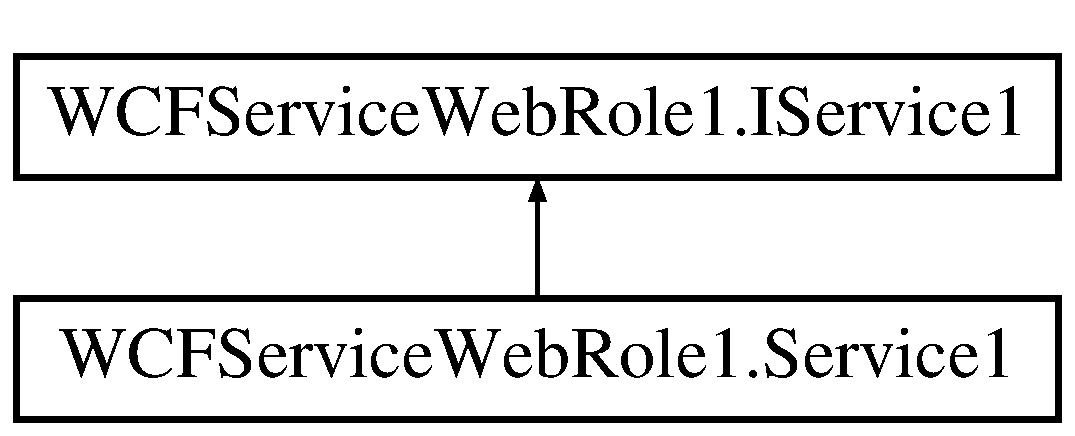
\includegraphics[height=2.000000cm]{interface_w_c_f_service_web_role1_1_1_i_service1}
\end{center}
\end{figure}
\subsection*{Public Member Functions}
\begin{DoxyCompactItemize}
\item 
\hypertarget{interface_w_c_f_service_web_role1_1_1_i_service1_a8f00ee69713054a16d9ca49c36894e1c}{}bool {\bfseries Check\+Database\+Connection} ()\label{interface_w_c_f_service_web_role1_1_1_i_service1_a8f00ee69713054a16d9ca49c36894e1c}

\item 
\hypertarget{interface_w_c_f_service_web_role1_1_1_i_service1_ab110be3e5449ab4a054da01efca9d4af}{}List$<$ \hyperlink{class_w_c_f_service_web_role1_1_1_measurement}{Measurement} $>$ {\bfseries Get\+Fifty\+Measurements\+From\+Room} (int room\+Id)\label{interface_w_c_f_service_web_role1_1_1_i_service1_ab110be3e5449ab4a054da01efca9d4af}

\item 
\hypertarget{interface_w_c_f_service_web_role1_1_1_i_service1_a2f9c519200ba30529289f7c0a7fe011b}{}List$<$ \hyperlink{class_w_c_f_service_web_role1_1_1_measurement}{Measurement} $>$ {\bfseries Get\+Latest\+Fifty\+Measurements\+From\+All} ()\label{interface_w_c_f_service_web_role1_1_1_i_service1_a2f9c519200ba30529289f7c0a7fe011b}

\item 
\hypertarget{interface_w_c_f_service_web_role1_1_1_i_service1_a6b5d59c027f59fee7fa0c93f31faddc0}{}List$<$ \hyperlink{class_w_c_f_service_web_role1_1_1_measurement}{Measurement} $>$ {\bfseries Get\+Measurements\+From\+Date} (Date\+Time from\+Date, Date\+Time to\+Date, int room\+Id)\label{interface_w_c_f_service_web_role1_1_1_i_service1_a6b5d59c027f59fee7fa0c93f31faddc0}

\item 
\hypertarget{interface_w_c_f_service_web_role1_1_1_i_service1_a0f98f8ace348304de3344629ae92a641}{}Dictionary$<$ string, \hyperlink{class_w_c_f_service_web_role1_1_1_measurement}{Measurement} $>$ {\bfseries Get\+Latest\+Measurements} ()\label{interface_w_c_f_service_web_role1_1_1_i_service1_a0f98f8ace348304de3344629ae92a641}

\item 
\hypertarget{interface_w_c_f_service_web_role1_1_1_i_service1_a0e5d931c3553c9e6d03c8a63c8fd9101}{}List$<$ \hyperlink{class_w_c_f_service_web_role1_1_1_room}{Room} $>$ {\bfseries Get\+Rooms} ()\label{interface_w_c_f_service_web_role1_1_1_i_service1_a0e5d931c3553c9e6d03c8a63c8fd9101}

\item 
\hypertarget{interface_w_c_f_service_web_role1_1_1_i_service1_aceea31eb37174848da60e96ff5e30dad}{}List$<$ \hyperlink{class_w_c_f_service_web_role1_1_1_room}{Room} $>$ {\bfseries Get\+Rooms\+By\+Temp} (double temperature, bool above=true)\label{interface_w_c_f_service_web_role1_1_1_i_service1_aceea31eb37174848da60e96ff5e30dad}

\item 
\hypertarget{interface_w_c_f_service_web_role1_1_1_i_service1_a16c69dc1cffb79158a160888bdeea8af}{}List$<$ \hyperlink{class_w_c_f_service_web_role1_1_1_room}{Room} $>$ {\bfseries Get\+Rooms\+By\+Date} (Date\+Time date, bool above=true)\label{interface_w_c_f_service_web_role1_1_1_i_service1_a16c69dc1cffb79158a160888bdeea8af}

\item 
\hypertarget{interface_w_c_f_service_web_role1_1_1_i_service1_ac8257abf679c212854debc3dfd2d1bf0}{}\hyperlink{class_w_c_f_service_web_role1_1_1_measurement}{Measurement} {\bfseries Insert\+Measurement} (\hyperlink{class_w_c_f_service_web_role1_1_1_measurement}{Measurement} measurement)\label{interface_w_c_f_service_web_role1_1_1_i_service1_ac8257abf679c212854debc3dfd2d1bf0}

\item 
\hypertarget{interface_w_c_f_service_web_role1_1_1_i_service1_aaa639c48573356f49aae7c6260b91eca}{}\hyperlink{class_w_c_f_service_web_role1_1_1_measurement}{Measurement} {\bfseries Delete\+Measurement} (\hyperlink{class_w_c_f_service_web_role1_1_1_measurement}{Measurement} measurement)\label{interface_w_c_f_service_web_role1_1_1_i_service1_aaa639c48573356f49aae7c6260b91eca}

\item 
\hypertarget{interface_w_c_f_service_web_role1_1_1_i_service1_a7398a7af401e117fd968f55ff0885642}{}\hyperlink{class_w_c_f_service_web_role1_1_1_room}{Room} {\bfseries Insert\+Room} (\hyperlink{class_w_c_f_service_web_role1_1_1_room}{Room} room)\label{interface_w_c_f_service_web_role1_1_1_i_service1_a7398a7af401e117fd968f55ff0885642}

\item 
\hypertarget{interface_w_c_f_service_web_role1_1_1_i_service1_abab37e67560089b43240544d04c4f1c3}{}\hyperlink{class_w_c_f_service_web_role1_1_1_room}{Room} {\bfseries Update\+Room} (int room\+Id, \hyperlink{class_w_c_f_service_web_role1_1_1_room}{Room} new\+Room)\label{interface_w_c_f_service_web_role1_1_1_i_service1_abab37e67560089b43240544d04c4f1c3}

\item 
\hypertarget{interface_w_c_f_service_web_role1_1_1_i_service1_a69a8714ed93d83d0bf623a118822d5f5}{}\hyperlink{class_w_c_f_service_web_role1_1_1_room}{Room} {\bfseries Delete\+Room} (int room\+Id)\label{interface_w_c_f_service_web_role1_1_1_i_service1_a69a8714ed93d83d0bf623a118822d5f5}

\end{DoxyCompactItemize}


The documentation for this interface was generated from the following file\+:\begin{DoxyCompactItemize}
\item 
C\+:/\+Users/\+Danny/\+Documents/\+Git\+Hub/3.-\/\+Semester-\/\+Environmentalist/\+W\+C\+F\+Service\+Web\+Role1/I\+Service1.\+cs\end{DoxyCompactItemize}

\hypertarget{class_w_c_f_service_web_role1_1_1_measurement}{}\section{W\+C\+F\+Service\+Web\+Role1.\+Measurement Class Reference}
\label{class_w_c_f_service_web_role1_1_1_measurement}\index{W\+C\+F\+Service\+Web\+Role1.\+Measurement@{W\+C\+F\+Service\+Web\+Role1.\+Measurement}}
\subsection*{Properties}
\begin{DoxyCompactItemize}
\item 
int \hyperlink{class_w_c_f_service_web_role1_1_1_measurement_a80bef1e085de826a7c693516b912c136}{Id}\hspace{0.3cm}{\ttfamily  \mbox{[}get, set\mbox{]}}
\begin{DoxyCompactList}\small\item\em The id of the measurement. Can be left as null. \end{DoxyCompactList}\item 
int \hyperlink{class_w_c_f_service_web_role1_1_1_measurement_a37bf0a9d6b3b2aecd532a4de45cc2076}{Room}\hspace{0.3cm}{\ttfamily  \mbox{[}get, set\mbox{]}}
\begin{DoxyCompactList}\small\item\em The id of the room the measurement belongs to. \end{DoxyCompactList}\item 
double \hyperlink{class_w_c_f_service_web_role1_1_1_measurement_a27481694219bde22fd509f9ada61fce6}{Temperature}\hspace{0.3cm}{\ttfamily  \mbox{[}get, set\mbox{]}}
\begin{DoxyCompactList}\small\item\em The temperature of the room. \end{DoxyCompactList}\item 
Date\+Time \hyperlink{class_w_c_f_service_web_role1_1_1_measurement_a7adec3362734460f2f2106401f496c41}{Movement}\hspace{0.3cm}{\ttfamily  \mbox{[}get, set\mbox{]}}
\begin{DoxyCompactList}\small\item\em The date and time when movement was last detected in the room. \end{DoxyCompactList}\item 
Date\+Time \hyperlink{class_w_c_f_service_web_role1_1_1_measurement_a40c9b7acb1a4bf2fe9b1a76cb3b0bfb1}{Date}\hspace{0.3cm}{\ttfamily  \mbox{[}get, set\mbox{]}}
\begin{DoxyCompactList}\small\item\em The date and time for the latest movement detection. \end{DoxyCompactList}\end{DoxyCompactItemize}


\subsection{Property Documentation}
\hypertarget{class_w_c_f_service_web_role1_1_1_measurement_a40c9b7acb1a4bf2fe9b1a76cb3b0bfb1}{}\index{W\+C\+F\+Service\+Web\+Role1\+::\+Measurement@{W\+C\+F\+Service\+Web\+Role1\+::\+Measurement}!Date@{Date}}
\index{Date@{Date}!W\+C\+F\+Service\+Web\+Role1\+::\+Measurement@{W\+C\+F\+Service\+Web\+Role1\+::\+Measurement}}
\subsubsection[{Date}]{\setlength{\rightskip}{0pt plus 5cm}Date\+Time W\+C\+F\+Service\+Web\+Role1.\+Measurement.\+Date\hspace{0.3cm}{\ttfamily [get]}, {\ttfamily [set]}}\label{class_w_c_f_service_web_role1_1_1_measurement_a40c9b7acb1a4bf2fe9b1a76cb3b0bfb1}


The date and time for the latest movement detection. 

\hypertarget{class_w_c_f_service_web_role1_1_1_measurement_a80bef1e085de826a7c693516b912c136}{}\index{W\+C\+F\+Service\+Web\+Role1\+::\+Measurement@{W\+C\+F\+Service\+Web\+Role1\+::\+Measurement}!Id@{Id}}
\index{Id@{Id}!W\+C\+F\+Service\+Web\+Role1\+::\+Measurement@{W\+C\+F\+Service\+Web\+Role1\+::\+Measurement}}
\subsubsection[{Id}]{\setlength{\rightskip}{0pt plus 5cm}int W\+C\+F\+Service\+Web\+Role1.\+Measurement.\+Id\hspace{0.3cm}{\ttfamily [get]}, {\ttfamily [set]}}\label{class_w_c_f_service_web_role1_1_1_measurement_a80bef1e085de826a7c693516b912c136}


The id of the measurement. Can be left as null. 

\hypertarget{class_w_c_f_service_web_role1_1_1_measurement_a7adec3362734460f2f2106401f496c41}{}\index{W\+C\+F\+Service\+Web\+Role1\+::\+Measurement@{W\+C\+F\+Service\+Web\+Role1\+::\+Measurement}!Movement@{Movement}}
\index{Movement@{Movement}!W\+C\+F\+Service\+Web\+Role1\+::\+Measurement@{W\+C\+F\+Service\+Web\+Role1\+::\+Measurement}}
\subsubsection[{Movement}]{\setlength{\rightskip}{0pt plus 5cm}Date\+Time W\+C\+F\+Service\+Web\+Role1.\+Measurement.\+Movement\hspace{0.3cm}{\ttfamily [get]}, {\ttfamily [set]}}\label{class_w_c_f_service_web_role1_1_1_measurement_a7adec3362734460f2f2106401f496c41}


The date and time when movement was last detected in the room. 

\hypertarget{class_w_c_f_service_web_role1_1_1_measurement_a37bf0a9d6b3b2aecd532a4de45cc2076}{}\index{W\+C\+F\+Service\+Web\+Role1\+::\+Measurement@{W\+C\+F\+Service\+Web\+Role1\+::\+Measurement}!Room@{Room}}
\index{Room@{Room}!W\+C\+F\+Service\+Web\+Role1\+::\+Measurement@{W\+C\+F\+Service\+Web\+Role1\+::\+Measurement}}
\subsubsection[{Room}]{\setlength{\rightskip}{0pt plus 5cm}int W\+C\+F\+Service\+Web\+Role1.\+Measurement.\+Room\hspace{0.3cm}{\ttfamily [get]}, {\ttfamily [set]}}\label{class_w_c_f_service_web_role1_1_1_measurement_a37bf0a9d6b3b2aecd532a4de45cc2076}


The id of the room the measurement belongs to. 

\hypertarget{class_w_c_f_service_web_role1_1_1_measurement_a27481694219bde22fd509f9ada61fce6}{}\index{W\+C\+F\+Service\+Web\+Role1\+::\+Measurement@{W\+C\+F\+Service\+Web\+Role1\+::\+Measurement}!Temperature@{Temperature}}
\index{Temperature@{Temperature}!W\+C\+F\+Service\+Web\+Role1\+::\+Measurement@{W\+C\+F\+Service\+Web\+Role1\+::\+Measurement}}
\subsubsection[{Temperature}]{\setlength{\rightskip}{0pt plus 5cm}double W\+C\+F\+Service\+Web\+Role1.\+Measurement.\+Temperature\hspace{0.3cm}{\ttfamily [get]}, {\ttfamily [set]}}\label{class_w_c_f_service_web_role1_1_1_measurement_a27481694219bde22fd509f9ada61fce6}


The temperature of the room. 



The documentation for this class was generated from the following file\+:\begin{DoxyCompactItemize}
\item 
C\+:/\+Users/\+Danny/\+Documents/\+Git\+Hub/3.-\/\+Semester-\/\+Environmentalist/\+W\+C\+F\+Service\+Web\+Role1/I\+Service1.\+cs\end{DoxyCompactItemize}

\hypertarget{class_w_c_f_service_web_role1_1_1_room}{}\section{W\+C\+F\+Service\+Web\+Role1.\+Room Class Reference}
\label{class_w_c_f_service_web_role1_1_1_room}\index{W\+C\+F\+Service\+Web\+Role1.\+Room@{W\+C\+F\+Service\+Web\+Role1.\+Room}}
\subsection*{Properties}
\begin{DoxyCompactItemize}
\item 
int \hyperlink{class_w_c_f_service_web_role1_1_1_room_a732db4bf7a1478e9c1a562f9f43f678a}{Id}\hspace{0.3cm}{\ttfamily  \mbox{[}get, set\mbox{]}}
\begin{DoxyCompactList}\small\item\em The id of the room. \end{DoxyCompactList}\item 
string \hyperlink{class_w_c_f_service_web_role1_1_1_room_ae1873490e3785fb100de49c6ac02edb5}{Name}\hspace{0.3cm}{\ttfamily  \mbox{[}get, set\mbox{]}}
\begin{DoxyCompactList}\small\item\em The name of the room. \end{DoxyCompactList}\end{DoxyCompactItemize}


\subsection{Property Documentation}
\hypertarget{class_w_c_f_service_web_role1_1_1_room_a732db4bf7a1478e9c1a562f9f43f678a}{}\index{W\+C\+F\+Service\+Web\+Role1\+::\+Room@{W\+C\+F\+Service\+Web\+Role1\+::\+Room}!Id@{Id}}
\index{Id@{Id}!W\+C\+F\+Service\+Web\+Role1\+::\+Room@{W\+C\+F\+Service\+Web\+Role1\+::\+Room}}
\subsubsection[{Id}]{\setlength{\rightskip}{0pt plus 5cm}int W\+C\+F\+Service\+Web\+Role1.\+Room.\+Id\hspace{0.3cm}{\ttfamily [get]}, {\ttfamily [set]}}\label{class_w_c_f_service_web_role1_1_1_room_a732db4bf7a1478e9c1a562f9f43f678a}


The id of the room. 

\hypertarget{class_w_c_f_service_web_role1_1_1_room_ae1873490e3785fb100de49c6ac02edb5}{}\index{W\+C\+F\+Service\+Web\+Role1\+::\+Room@{W\+C\+F\+Service\+Web\+Role1\+::\+Room}!Name@{Name}}
\index{Name@{Name}!W\+C\+F\+Service\+Web\+Role1\+::\+Room@{W\+C\+F\+Service\+Web\+Role1\+::\+Room}}
\subsubsection[{Name}]{\setlength{\rightskip}{0pt plus 5cm}string W\+C\+F\+Service\+Web\+Role1.\+Room.\+Name\hspace{0.3cm}{\ttfamily [get]}, {\ttfamily [set]}}\label{class_w_c_f_service_web_role1_1_1_room_ae1873490e3785fb100de49c6ac02edb5}


The name of the room. 



The documentation for this class was generated from the following file\+:\begin{DoxyCompactItemize}
\item 
C\+:/\+Users/\+Danny/\+Documents/\+Git\+Hub/3.-\/\+Semester-\/\+Environmentalist/\+W\+C\+F\+Service\+Web\+Role1/I\+Service1.\+cs\end{DoxyCompactItemize}

\hypertarget{class_w_c_f_service_web_role1_1_1_service1}{}\section{W\+C\+F\+Service\+Web\+Role1.\+Service1 Class Reference}
\label{class_w_c_f_service_web_role1_1_1_service1}\index{W\+C\+F\+Service\+Web\+Role1.\+Service1@{W\+C\+F\+Service\+Web\+Role1.\+Service1}}
Inheritance diagram for W\+C\+F\+Service\+Web\+Role1.\+Service1\+:\begin{figure}[H]
\begin{center}
\leavevmode
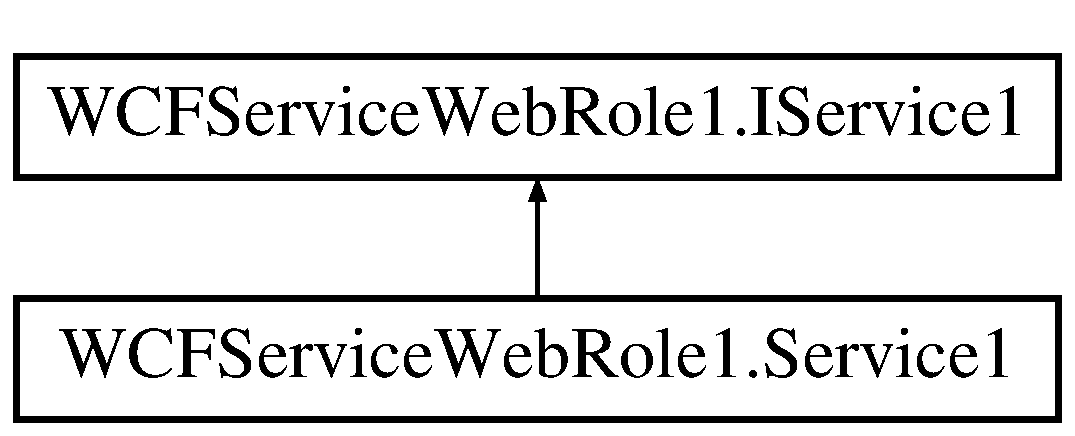
\includegraphics[height=2.000000cm]{class_w_c_f_service_web_role1_1_1_service1}
\end{center}
\end{figure}
\subsection*{Public Member Functions}
\begin{DoxyCompactItemize}
\item 
\hyperlink{class_w_c_f_service_web_role1_1_1_service1_a2db81b21b72abb231eebe975e129edc3}{Service1} ()
\begin{DoxyCompactList}\small\item\em Constructor used to initialize and establish S\+Q\+L-\/connection to the database, while also setting up tracing. \end{DoxyCompactList}\item 
bool \hyperlink{class_w_c_f_service_web_role1_1_1_service1_ab9f6ac135248447bd6546a3bb1cf042e}{Check\+Database\+Connection} ()
\begin{DoxyCompactList}\small\item\em Testmethod to ensure correct connection to the database. \end{DoxyCompactList}\item 
List$<$ \hyperlink{class_w_c_f_service_web_role1_1_1_measurement}{Measurement} $>$ \hyperlink{class_w_c_f_service_web_role1_1_1_service1_ab890a11f44c88ed8cabd4b441e28abb7}{Get\+Fifty\+Measurements\+From\+Room} (int room\+Id)
\begin{DoxyCompactList}\small\item\em Returns the latest fifty measurements from the specified room. \end{DoxyCompactList}\item 
List$<$ \hyperlink{class_w_c_f_service_web_role1_1_1_measurement}{Measurement} $>$ \hyperlink{class_w_c_f_service_web_role1_1_1_service1_ac5bb626b88cb7f56a06cd5e8eeeb79ab}{Get\+Measurements\+From\+Date} (Date\+Time from\+Date, Date\+Time to\+Date, int room\+Id)
\begin{DoxyCompactList}\small\item\em Returns all measurements between the specified dates from the room with the specified id. \end{DoxyCompactList}\item 
Dictionary$<$ string, \hyperlink{class_w_c_f_service_web_role1_1_1_measurement}{Measurement} $>$ \hyperlink{class_w_c_f_service_web_role1_1_1_service1_a1dadae6d813e21bf454f3ef00741b32d}{Get\+Latest\+Measurements} ()
\begin{DoxyCompactList}\small\item\em Returns the single latest measurement from all rooms. \end{DoxyCompactList}\item 
List$<$ \hyperlink{class_w_c_f_service_web_role1_1_1_measurement}{Measurement} $>$ \hyperlink{class_w_c_f_service_web_role1_1_1_service1_afe243908ef6a247439b92823d04d1108}{Get\+Latest\+Fifty\+Measurements\+From\+All} ()
\begin{DoxyCompactList}\small\item\em Returns the fifty latest measurements from all rooms. \end{DoxyCompactList}\item 
List$<$ \hyperlink{class_w_c_f_service_web_role1_1_1_room}{Room} $>$ \hyperlink{class_w_c_f_service_web_role1_1_1_service1_a5534cff1f8e4868d5f55380da04b3a7a}{Get\+Rooms} ()
\begin{DoxyCompactList}\small\item\em Returns all rooms. \end{DoxyCompactList}\item 
List$<$ \hyperlink{class_w_c_f_service_web_role1_1_1_room}{Room} $>$ \hyperlink{class_w_c_f_service_web_role1_1_1_service1_a085108986fe8820c44e8dcad62750cec}{Get\+Rooms\+By\+Temp} (double temperature, bool above=true)
\begin{DoxyCompactList}\small\item\em Returns all rooms above/below the specified temperature. \end{DoxyCompactList}\item 
List$<$ \hyperlink{class_w_c_f_service_web_role1_1_1_room}{Room} $>$ \hyperlink{class_w_c_f_service_web_role1_1_1_service1_afd71e5b1f7aad89f3655eb9c265c3705}{Get\+Rooms\+By\+Date} (Date\+Time date, bool after=true)
\begin{DoxyCompactList}\small\item\em Returns all rooms with detected movement after/before the specified date. \end{DoxyCompactList}\item 
\hyperlink{class_w_c_f_service_web_role1_1_1_measurement}{Measurement} \hyperlink{class_w_c_f_service_web_role1_1_1_service1_a91cca3523909a15506670a99f0a13739}{Insert\+Measurement} (\hyperlink{class_w_c_f_service_web_role1_1_1_measurement}{Measurement} measurement)
\begin{DoxyCompactList}\small\item\em Inserts the specified \hyperlink{class_w_c_f_service_web_role1_1_1_measurement}{Measurement} object into the database. \end{DoxyCompactList}\item 
\hyperlink{class_w_c_f_service_web_role1_1_1_measurement}{Measurement} \hyperlink{class_w_c_f_service_web_role1_1_1_service1_a0a05f8caeea4bfc3fb5e9675ae0a04e8}{Delete\+Measurement} (\hyperlink{class_w_c_f_service_web_role1_1_1_measurement}{Measurement} measurement)
\begin{DoxyCompactList}\small\item\em Deletes the specified \hyperlink{class_w_c_f_service_web_role1_1_1_measurement}{Measurement} object from the database. \end{DoxyCompactList}\item 
\hyperlink{class_w_c_f_service_web_role1_1_1_room}{Room} \hyperlink{class_w_c_f_service_web_role1_1_1_service1_a03546c5dac6e980720ecad385039e083}{Insert\+Room} (\hyperlink{class_w_c_f_service_web_role1_1_1_room}{Room} room)
\begin{DoxyCompactList}\small\item\em Inserts the specified \hyperlink{class_w_c_f_service_web_role1_1_1_room}{Room} object into the database. \end{DoxyCompactList}\item 
\hyperlink{class_w_c_f_service_web_role1_1_1_room}{Room} \hyperlink{class_w_c_f_service_web_role1_1_1_service1_a0d512fc6b1525964695786a336058c04}{Update\+Room} (int room\+Id, \hyperlink{class_w_c_f_service_web_role1_1_1_room}{Room} new\+Room)
\begin{DoxyCompactList}\small\item\em Updates the specified room with the new specfied \hyperlink{class_w_c_f_service_web_role1_1_1_room}{Room} object. \end{DoxyCompactList}\item 
\hyperlink{class_w_c_f_service_web_role1_1_1_room}{Room} \hyperlink{class_w_c_f_service_web_role1_1_1_service1_abd3f431c0a5cc6138351ae81cb955286}{Delete\+Room} (int room\+Id)
\begin{DoxyCompactList}\small\item\em Deletes the specified room from the database. \end{DoxyCompactList}\end{DoxyCompactItemize}


\subsection{Constructor \& Destructor Documentation}
\hypertarget{class_w_c_f_service_web_role1_1_1_service1_a2db81b21b72abb231eebe975e129edc3}{}\index{W\+C\+F\+Service\+Web\+Role1\+::\+Service1@{W\+C\+F\+Service\+Web\+Role1\+::\+Service1}!Service1@{Service1}}
\index{Service1@{Service1}!W\+C\+F\+Service\+Web\+Role1\+::\+Service1@{W\+C\+F\+Service\+Web\+Role1\+::\+Service1}}
\subsubsection[{Service1()}]{\setlength{\rightskip}{0pt plus 5cm}W\+C\+F\+Service\+Web\+Role1.\+Service1.\+Service1 (
\begin{DoxyParamCaption}
{}
\end{DoxyParamCaption}
)}\label{class_w_c_f_service_web_role1_1_1_service1_a2db81b21b72abb231eebe975e129edc3}


Constructor used to initialize and establish S\+Q\+L-\/connection to the database, while also setting up tracing. 



\subsection{Member Function Documentation}
\hypertarget{class_w_c_f_service_web_role1_1_1_service1_ab9f6ac135248447bd6546a3bb1cf042e}{}\index{W\+C\+F\+Service\+Web\+Role1\+::\+Service1@{W\+C\+F\+Service\+Web\+Role1\+::\+Service1}!Check\+Database\+Connection@{Check\+Database\+Connection}}
\index{Check\+Database\+Connection@{Check\+Database\+Connection}!W\+C\+F\+Service\+Web\+Role1\+::\+Service1@{W\+C\+F\+Service\+Web\+Role1\+::\+Service1}}
\subsubsection[{Check\+Database\+Connection()}]{\setlength{\rightskip}{0pt plus 5cm}bool W\+C\+F\+Service\+Web\+Role1.\+Service1.\+Check\+Database\+Connection (
\begin{DoxyParamCaption}
{}
\end{DoxyParamCaption}
)}\label{class_w_c_f_service_web_role1_1_1_service1_ab9f6ac135248447bd6546a3bb1cf042e}


Testmethod to ensure correct connection to the database. 

\begin{DoxyReturn}{Returns}

\end{DoxyReturn}


Implements \hyperlink{interface_w_c_f_service_web_role1_1_1_i_service1}{W\+C\+F\+Service\+Web\+Role1.\+I\+Service1}.

\hypertarget{class_w_c_f_service_web_role1_1_1_service1_a0a05f8caeea4bfc3fb5e9675ae0a04e8}{}\index{W\+C\+F\+Service\+Web\+Role1\+::\+Service1@{W\+C\+F\+Service\+Web\+Role1\+::\+Service1}!Delete\+Measurement@{Delete\+Measurement}}
\index{Delete\+Measurement@{Delete\+Measurement}!W\+C\+F\+Service\+Web\+Role1\+::\+Service1@{W\+C\+F\+Service\+Web\+Role1\+::\+Service1}}
\subsubsection[{Delete\+Measurement(\+Measurement measurement)}]{\setlength{\rightskip}{0pt plus 5cm}{\bf Measurement} W\+C\+F\+Service\+Web\+Role1.\+Service1.\+Delete\+Measurement (
\begin{DoxyParamCaption}
\item[{{\bf Measurement}}]{measurement}
\end{DoxyParamCaption}
)}\label{class_w_c_f_service_web_role1_1_1_service1_a0a05f8caeea4bfc3fb5e9675ae0a04e8}


Deletes the specified \hyperlink{class_w_c_f_service_web_role1_1_1_measurement}{Measurement} object from the database. 


\begin{DoxyParams}{Parameters}
{\em measurement} & The \hyperlink{class_w_c_f_service_web_role1_1_1_measurement}{Measurement} to remove from the database.\\
\hline
\end{DoxyParams}
\begin{DoxyReturn}{Returns}

\end{DoxyReturn}


Implements \hyperlink{interface_w_c_f_service_web_role1_1_1_i_service1}{W\+C\+F\+Service\+Web\+Role1.\+I\+Service1}.

\hypertarget{class_w_c_f_service_web_role1_1_1_service1_abd3f431c0a5cc6138351ae81cb955286}{}\index{W\+C\+F\+Service\+Web\+Role1\+::\+Service1@{W\+C\+F\+Service\+Web\+Role1\+::\+Service1}!Delete\+Room@{Delete\+Room}}
\index{Delete\+Room@{Delete\+Room}!W\+C\+F\+Service\+Web\+Role1\+::\+Service1@{W\+C\+F\+Service\+Web\+Role1\+::\+Service1}}
\subsubsection[{Delete\+Room(int room\+Id)}]{\setlength{\rightskip}{0pt plus 5cm}{\bf Room} W\+C\+F\+Service\+Web\+Role1.\+Service1.\+Delete\+Room (
\begin{DoxyParamCaption}
\item[{int}]{room\+Id}
\end{DoxyParamCaption}
)}\label{class_w_c_f_service_web_role1_1_1_service1_abd3f431c0a5cc6138351ae81cb955286}


Deletes the specified room from the database. 


\begin{DoxyParams}{Parameters}
{\em room\+Id} & The id of the room to remove from the database.\\
\hline
\end{DoxyParams}
\begin{DoxyReturn}{Returns}

\end{DoxyReturn}


Implements \hyperlink{interface_w_c_f_service_web_role1_1_1_i_service1}{W\+C\+F\+Service\+Web\+Role1.\+I\+Service1}.

\hypertarget{class_w_c_f_service_web_role1_1_1_service1_ab890a11f44c88ed8cabd4b441e28abb7}{}\index{W\+C\+F\+Service\+Web\+Role1\+::\+Service1@{W\+C\+F\+Service\+Web\+Role1\+::\+Service1}!Get\+Fifty\+Measurements\+From\+Room@{Get\+Fifty\+Measurements\+From\+Room}}
\index{Get\+Fifty\+Measurements\+From\+Room@{Get\+Fifty\+Measurements\+From\+Room}!W\+C\+F\+Service\+Web\+Role1\+::\+Service1@{W\+C\+F\+Service\+Web\+Role1\+::\+Service1}}
\subsubsection[{Get\+Fifty\+Measurements\+From\+Room(int room\+Id)}]{\setlength{\rightskip}{0pt plus 5cm}List$<${\bf Measurement}$>$ W\+C\+F\+Service\+Web\+Role1.\+Service1.\+Get\+Fifty\+Measurements\+From\+Room (
\begin{DoxyParamCaption}
\item[{int}]{room\+Id}
\end{DoxyParamCaption}
)}\label{class_w_c_f_service_web_role1_1_1_service1_ab890a11f44c88ed8cabd4b441e28abb7}


Returns the latest fifty measurements from the specified room. 


\begin{DoxyParams}{Parameters}
{\em room\+Id} & Id of the room to get latest fifty measurements from.\\
\hline
\end{DoxyParams}
\begin{DoxyReturn}{Returns}

\end{DoxyReturn}


Implements \hyperlink{interface_w_c_f_service_web_role1_1_1_i_service1}{W\+C\+F\+Service\+Web\+Role1.\+I\+Service1}.

\hypertarget{class_w_c_f_service_web_role1_1_1_service1_afe243908ef6a247439b92823d04d1108}{}\index{W\+C\+F\+Service\+Web\+Role1\+::\+Service1@{W\+C\+F\+Service\+Web\+Role1\+::\+Service1}!Get\+Latest\+Fifty\+Measurements\+From\+All@{Get\+Latest\+Fifty\+Measurements\+From\+All}}
\index{Get\+Latest\+Fifty\+Measurements\+From\+All@{Get\+Latest\+Fifty\+Measurements\+From\+All}!W\+C\+F\+Service\+Web\+Role1\+::\+Service1@{W\+C\+F\+Service\+Web\+Role1\+::\+Service1}}
\subsubsection[{Get\+Latest\+Fifty\+Measurements\+From\+All()}]{\setlength{\rightskip}{0pt plus 5cm}List$<${\bf Measurement}$>$ W\+C\+F\+Service\+Web\+Role1.\+Service1.\+Get\+Latest\+Fifty\+Measurements\+From\+All (
\begin{DoxyParamCaption}
{}
\end{DoxyParamCaption}
)}\label{class_w_c_f_service_web_role1_1_1_service1_afe243908ef6a247439b92823d04d1108}


Returns the fifty latest measurements from all rooms. 

\begin{DoxyReturn}{Returns}

\end{DoxyReturn}


Implements \hyperlink{interface_w_c_f_service_web_role1_1_1_i_service1}{W\+C\+F\+Service\+Web\+Role1.\+I\+Service1}.

\hypertarget{class_w_c_f_service_web_role1_1_1_service1_a1dadae6d813e21bf454f3ef00741b32d}{}\index{W\+C\+F\+Service\+Web\+Role1\+::\+Service1@{W\+C\+F\+Service\+Web\+Role1\+::\+Service1}!Get\+Latest\+Measurements@{Get\+Latest\+Measurements}}
\index{Get\+Latest\+Measurements@{Get\+Latest\+Measurements}!W\+C\+F\+Service\+Web\+Role1\+::\+Service1@{W\+C\+F\+Service\+Web\+Role1\+::\+Service1}}
\subsubsection[{Get\+Latest\+Measurements()}]{\setlength{\rightskip}{0pt plus 5cm}Dictionary$<$string, {\bf Measurement}$>$ W\+C\+F\+Service\+Web\+Role1.\+Service1.\+Get\+Latest\+Measurements (
\begin{DoxyParamCaption}
{}
\end{DoxyParamCaption}
)}\label{class_w_c_f_service_web_role1_1_1_service1_a1dadae6d813e21bf454f3ef00741b32d}


Returns the single latest measurement from all rooms. 

\begin{DoxyReturn}{Returns}

\end{DoxyReturn}


Implements \hyperlink{interface_w_c_f_service_web_role1_1_1_i_service1}{W\+C\+F\+Service\+Web\+Role1.\+I\+Service1}.

\hypertarget{class_w_c_f_service_web_role1_1_1_service1_ac5bb626b88cb7f56a06cd5e8eeeb79ab}{}\index{W\+C\+F\+Service\+Web\+Role1\+::\+Service1@{W\+C\+F\+Service\+Web\+Role1\+::\+Service1}!Get\+Measurements\+From\+Date@{Get\+Measurements\+From\+Date}}
\index{Get\+Measurements\+From\+Date@{Get\+Measurements\+From\+Date}!W\+C\+F\+Service\+Web\+Role1\+::\+Service1@{W\+C\+F\+Service\+Web\+Role1\+::\+Service1}}
\subsubsection[{Get\+Measurements\+From\+Date(\+Date\+Time from\+Date, Date\+Time to\+Date, int room\+Id)}]{\setlength{\rightskip}{0pt plus 5cm}List$<${\bf Measurement}$>$ W\+C\+F\+Service\+Web\+Role1.\+Service1.\+Get\+Measurements\+From\+Date (
\begin{DoxyParamCaption}
\item[{Date\+Time}]{from\+Date, }
\item[{Date\+Time}]{to\+Date, }
\item[{int}]{room\+Id}
\end{DoxyParamCaption}
)}\label{class_w_c_f_service_web_role1_1_1_service1_ac5bb626b88cb7f56a06cd5e8eeeb79ab}


Returns all measurements between the specified dates from the room with the specified id. 


\begin{DoxyParams}{Parameters}
{\em from\+Date} & From-\/date.\\
\hline
{\em to\+Date} & To-\/date.\\
\hline
{\em room\+Id} & Id of the room to get measurements from.\\
\hline
\end{DoxyParams}
\begin{DoxyReturn}{Returns}

\end{DoxyReturn}


Implements \hyperlink{interface_w_c_f_service_web_role1_1_1_i_service1}{W\+C\+F\+Service\+Web\+Role1.\+I\+Service1}.

\hypertarget{class_w_c_f_service_web_role1_1_1_service1_a5534cff1f8e4868d5f55380da04b3a7a}{}\index{W\+C\+F\+Service\+Web\+Role1\+::\+Service1@{W\+C\+F\+Service\+Web\+Role1\+::\+Service1}!Get\+Rooms@{Get\+Rooms}}
\index{Get\+Rooms@{Get\+Rooms}!W\+C\+F\+Service\+Web\+Role1\+::\+Service1@{W\+C\+F\+Service\+Web\+Role1\+::\+Service1}}
\subsubsection[{Get\+Rooms()}]{\setlength{\rightskip}{0pt plus 5cm}List$<${\bf Room}$>$ W\+C\+F\+Service\+Web\+Role1.\+Service1.\+Get\+Rooms (
\begin{DoxyParamCaption}
{}
\end{DoxyParamCaption}
)}\label{class_w_c_f_service_web_role1_1_1_service1_a5534cff1f8e4868d5f55380da04b3a7a}


Returns all rooms. 

\begin{DoxyReturn}{Returns}

\end{DoxyReturn}


Implements \hyperlink{interface_w_c_f_service_web_role1_1_1_i_service1}{W\+C\+F\+Service\+Web\+Role1.\+I\+Service1}.

\hypertarget{class_w_c_f_service_web_role1_1_1_service1_afd71e5b1f7aad89f3655eb9c265c3705}{}\index{W\+C\+F\+Service\+Web\+Role1\+::\+Service1@{W\+C\+F\+Service\+Web\+Role1\+::\+Service1}!Get\+Rooms\+By\+Date@{Get\+Rooms\+By\+Date}}
\index{Get\+Rooms\+By\+Date@{Get\+Rooms\+By\+Date}!W\+C\+F\+Service\+Web\+Role1\+::\+Service1@{W\+C\+F\+Service\+Web\+Role1\+::\+Service1}}
\subsubsection[{Get\+Rooms\+By\+Date(\+Date\+Time date, bool after=true)}]{\setlength{\rightskip}{0pt plus 5cm}List$<${\bf Room}$>$ W\+C\+F\+Service\+Web\+Role1.\+Service1.\+Get\+Rooms\+By\+Date (
\begin{DoxyParamCaption}
\item[{Date\+Time}]{date, }
\item[{bool}]{after = {\ttfamily true}}
\end{DoxyParamCaption}
)}\label{class_w_c_f_service_web_role1_1_1_service1_afd71e5b1f7aad89f3655eb9c265c3705}


Returns all rooms with detected movement after/before the specified date. 


\begin{DoxyParams}{Parameters}
{\em date} & Date.\\
\hline
{\em after} & If left true, the method returns the rooms that detected movement after the specified date. If set to false, the method returns the rooms that detected movement before the specified date.\\
\hline
\end{DoxyParams}
\begin{DoxyReturn}{Returns}

\end{DoxyReturn}


Implements \hyperlink{interface_w_c_f_service_web_role1_1_1_i_service1}{W\+C\+F\+Service\+Web\+Role1.\+I\+Service1}.

\hypertarget{class_w_c_f_service_web_role1_1_1_service1_a085108986fe8820c44e8dcad62750cec}{}\index{W\+C\+F\+Service\+Web\+Role1\+::\+Service1@{W\+C\+F\+Service\+Web\+Role1\+::\+Service1}!Get\+Rooms\+By\+Temp@{Get\+Rooms\+By\+Temp}}
\index{Get\+Rooms\+By\+Temp@{Get\+Rooms\+By\+Temp}!W\+C\+F\+Service\+Web\+Role1\+::\+Service1@{W\+C\+F\+Service\+Web\+Role1\+::\+Service1}}
\subsubsection[{Get\+Rooms\+By\+Temp(double temperature, bool above=true)}]{\setlength{\rightskip}{0pt plus 5cm}List$<${\bf Room}$>$ W\+C\+F\+Service\+Web\+Role1.\+Service1.\+Get\+Rooms\+By\+Temp (
\begin{DoxyParamCaption}
\item[{double}]{temperature, }
\item[{bool}]{above = {\ttfamily true}}
\end{DoxyParamCaption}
)}\label{class_w_c_f_service_web_role1_1_1_service1_a085108986fe8820c44e8dcad62750cec}


Returns all rooms above/below the specified temperature. 


\begin{DoxyParams}{Parameters}
{\em temperature} & Temperature.\\
\hline
{\em above} & If left true, the method returns the rooms above the specifed temperature. If set to false, the method returns the rooms below the specified temperature.\\
\hline
\end{DoxyParams}
\begin{DoxyReturn}{Returns}

\end{DoxyReturn}


Implements \hyperlink{interface_w_c_f_service_web_role1_1_1_i_service1}{W\+C\+F\+Service\+Web\+Role1.\+I\+Service1}.

\hypertarget{class_w_c_f_service_web_role1_1_1_service1_a91cca3523909a15506670a99f0a13739}{}\index{W\+C\+F\+Service\+Web\+Role1\+::\+Service1@{W\+C\+F\+Service\+Web\+Role1\+::\+Service1}!Insert\+Measurement@{Insert\+Measurement}}
\index{Insert\+Measurement@{Insert\+Measurement}!W\+C\+F\+Service\+Web\+Role1\+::\+Service1@{W\+C\+F\+Service\+Web\+Role1\+::\+Service1}}
\subsubsection[{Insert\+Measurement(\+Measurement measurement)}]{\setlength{\rightskip}{0pt plus 5cm}{\bf Measurement} W\+C\+F\+Service\+Web\+Role1.\+Service1.\+Insert\+Measurement (
\begin{DoxyParamCaption}
\item[{{\bf Measurement}}]{measurement}
\end{DoxyParamCaption}
)}\label{class_w_c_f_service_web_role1_1_1_service1_a91cca3523909a15506670a99f0a13739}


Inserts the specified \hyperlink{class_w_c_f_service_web_role1_1_1_measurement}{Measurement} object into the database. 


\begin{DoxyParams}{Parameters}
{\em measurement} & The \hyperlink{class_w_c_f_service_web_role1_1_1_measurement}{Measurement} to upload to the database.\\
\hline
\end{DoxyParams}
\begin{DoxyReturn}{Returns}

\end{DoxyReturn}


Implements \hyperlink{interface_w_c_f_service_web_role1_1_1_i_service1}{W\+C\+F\+Service\+Web\+Role1.\+I\+Service1}.

\hypertarget{class_w_c_f_service_web_role1_1_1_service1_a03546c5dac6e980720ecad385039e083}{}\index{W\+C\+F\+Service\+Web\+Role1\+::\+Service1@{W\+C\+F\+Service\+Web\+Role1\+::\+Service1}!Insert\+Room@{Insert\+Room}}
\index{Insert\+Room@{Insert\+Room}!W\+C\+F\+Service\+Web\+Role1\+::\+Service1@{W\+C\+F\+Service\+Web\+Role1\+::\+Service1}}
\subsubsection[{Insert\+Room(\+Room room)}]{\setlength{\rightskip}{0pt plus 5cm}{\bf Room} W\+C\+F\+Service\+Web\+Role1.\+Service1.\+Insert\+Room (
\begin{DoxyParamCaption}
\item[{{\bf Room}}]{room}
\end{DoxyParamCaption}
)}\label{class_w_c_f_service_web_role1_1_1_service1_a03546c5dac6e980720ecad385039e083}


Inserts the specified \hyperlink{class_w_c_f_service_web_role1_1_1_room}{Room} object into the database. 


\begin{DoxyParams}{Parameters}
{\em room} & The \hyperlink{class_w_c_f_service_web_role1_1_1_room}{Room} to upload to the database.\\
\hline
\end{DoxyParams}
\begin{DoxyReturn}{Returns}

\end{DoxyReturn}


Implements \hyperlink{interface_w_c_f_service_web_role1_1_1_i_service1}{W\+C\+F\+Service\+Web\+Role1.\+I\+Service1}.

\hypertarget{class_w_c_f_service_web_role1_1_1_service1_a0d512fc6b1525964695786a336058c04}{}\index{W\+C\+F\+Service\+Web\+Role1\+::\+Service1@{W\+C\+F\+Service\+Web\+Role1\+::\+Service1}!Update\+Room@{Update\+Room}}
\index{Update\+Room@{Update\+Room}!W\+C\+F\+Service\+Web\+Role1\+::\+Service1@{W\+C\+F\+Service\+Web\+Role1\+::\+Service1}}
\subsubsection[{Update\+Room(int room\+Id, Room new\+Room)}]{\setlength{\rightskip}{0pt plus 5cm}{\bf Room} W\+C\+F\+Service\+Web\+Role1.\+Service1.\+Update\+Room (
\begin{DoxyParamCaption}
\item[{int}]{room\+Id, }
\item[{{\bf Room}}]{new\+Room}
\end{DoxyParamCaption}
)}\label{class_w_c_f_service_web_role1_1_1_service1_a0d512fc6b1525964695786a336058c04}


Updates the specified room with the new specfied \hyperlink{class_w_c_f_service_web_role1_1_1_room}{Room} object. 


\begin{DoxyParams}{Parameters}
{\em room\+Id} & The id of the room to update.\\
\hline
{\em new\+Room} & The \hyperlink{class_w_c_f_service_web_role1_1_1_room}{Room} object to update to.\\
\hline
\end{DoxyParams}
\begin{DoxyReturn}{Returns}

\end{DoxyReturn}


Implements \hyperlink{interface_w_c_f_service_web_role1_1_1_i_service1}{W\+C\+F\+Service\+Web\+Role1.\+I\+Service1}.



The documentation for this class was generated from the following file\+:\begin{DoxyCompactItemize}
\item 
C\+:/\+Users/\+Danny/\+Documents/\+Git\+Hub/3.-\/\+Semester-\/\+Environmentalist/\+W\+C\+F\+Service\+Web\+Role1/Service1.\+svc.\+cs\end{DoxyCompactItemize}

\hypertarget{class_unit_test_project_1_1_unit_test1}{}\section{Unit\+Test\+Project.\+Unit\+Test1 Class Reference}
\label{class_unit_test_project_1_1_unit_test1}\index{Unit\+Test\+Project.\+Unit\+Test1@{Unit\+Test\+Project.\+Unit\+Test1}}
\subsection*{Public Member Functions}
\begin{DoxyCompactItemize}
\item 
\hypertarget{class_unit_test_project_1_1_unit_test1_a1cd53bf019a6a5ac0422147c8b1434da}{}void {\bfseries Test\+Method1} ()\label{class_unit_test_project_1_1_unit_test1_a1cd53bf019a6a5ac0422147c8b1434da}

\end{DoxyCompactItemize}


The documentation for this class was generated from the following file\+:\begin{DoxyCompactItemize}
\item 
C\+:/\+Users/\+Danny/\+Documents/\+Git\+Hub/3.-\/\+Semester-\/\+Environmentalist/\+Unit\+Test\+Project/Unit\+Test1.\+cs\end{DoxyCompactItemize}

\hypertarget{class_w_c_f_service_web_role1_1_1_web_role}{}\section{W\+C\+F\+Service\+Web\+Role1.\+Web\+Role Class Reference}
\label{class_w_c_f_service_web_role1_1_1_web_role}\index{W\+C\+F\+Service\+Web\+Role1.\+Web\+Role@{W\+C\+F\+Service\+Web\+Role1.\+Web\+Role}}
Inheritance diagram for W\+C\+F\+Service\+Web\+Role1.\+Web\+Role\+:\begin{figure}[H]
\begin{center}
\leavevmode
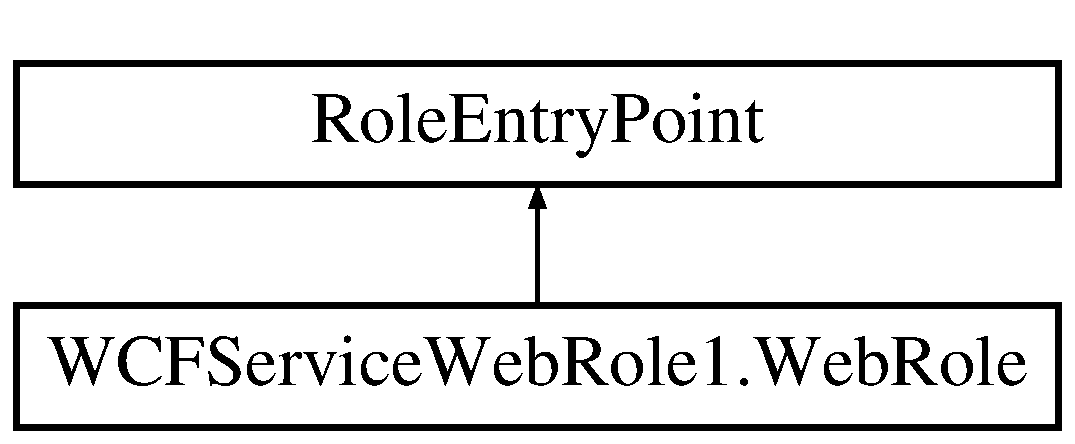
\includegraphics[height=2.000000cm]{class_w_c_f_service_web_role1_1_1_web_role}
\end{center}
\end{figure}
\subsection*{Public Member Functions}
\begin{DoxyCompactItemize}
\item 
\hypertarget{class_w_c_f_service_web_role1_1_1_web_role_a8c4c2d91db91aba6cb62a3a5e90d0002}{}override bool {\bfseries On\+Start} ()\label{class_w_c_f_service_web_role1_1_1_web_role_a8c4c2d91db91aba6cb62a3a5e90d0002}

\end{DoxyCompactItemize}


The documentation for this class was generated from the following file\+:\begin{DoxyCompactItemize}
\item 
C\+:/\+Users/\+Danny/\+Documents/\+Git\+Hub/3.-\/\+Semester-\/\+Environmentalist/\+W\+C\+F\+Service\+Web\+Role1/Web\+Role.\+cs\end{DoxyCompactItemize}

%--- End generated contents ---

% Index
\backmatter
\newpage
\phantomsection
\clearemptydoublepage
\addcontentsline{toc}{chapter}{Index}
\printindex

\end{document}
